%%%%%%%%%%%%%%%%%%%%%%%%%%%%%%%%%%%%%%%%%
% Engineering Calculation Paper
% LaTeX Template
% Version 1.0 (20/1/13)
%
% This template has been downloaded from:
% http://www.LaTeXTemplates.com
%
% Original author:
% Dmitry Volynkin (dim_voly@yahoo.com.au)
%
% License:
% CC BY-NC-SA 3.0 (http://creativecommons.org/licenses/by-nc-sa/3.0/)
%
%%%%%%%%%%%%%%%%%%%%%%%%%%%%%%%%%%%%%%%%%

%----------------------------------------------------------------------------------------
%	PACKAGES AND OTHER DOCUMENT CONFIGURATIONS
%----------------------------------------------------------------------------------------

\documentclass[12pt,a4paper]{article} % Use A4 paper with a 12pt font size - different paper sizes will require manual recalculation of page margins and border positions
\usepackage[utf8]{inputenc}
\usepackage{marginnote} % Required for margin notes
\usepackage{wallpaper} % Required to set each page to have a background
\usepackage[francais]{babel}
\usepackage{bclogo}
\usepackage{eurosym}
\usepackage{smartdiagram}
\usepackage{tikz}
\usetikzlibrary{quotes,angles}
\usetikzlibrary{calc,decorations.markings,fit}
\usetikzlibrary{trees,positioning,arrows,chains,shapes.geometric,decorations.pathreplacing,decorations.pathmorphing,shapes,matrix,shapes.symbols}
\usepackage{lastpage} % Required to print the total number of pages
\usepackage[left=1.3cm,right=4.6cm,top=1.8cm,bottom=4.0cm,marginparwidth=3.4cm]{geometry} % Adjust page margins
\usepackage{amsmath} % Required for equation customization
\usepackage{amssymb} % Required to include mathematical symbols
\usepackage{xcolor} % Required to specify colors by name

\usepackage{fancyhdr} % Required to customize headers
\setlength{\headheight}{80pt} % Increase the size of the header to accommodate meta-information
\pagestyle{fancy}\fancyhf{} % Use the custom header specified below
\renewcommand{\headrulewidth}{0pt} % Remove the default horizontal rule under the header

\setlength{\parindent}{0cm} % Remove paragraph indentation
\newcommand{\tab}{\hspace*{2em}} % Defines a new command for some horizontal space


%%%%%%%%%
%\renewcommand{\thesubsection}{[\Alph{section}](\alph{subsection})}
%%%%%%%%%

\newcommand\BackgroundStructure{ % Command to specify the background of each page
\setlength{\unitlength}{1mm} % Set the unit length to millimeters

\setlength\fboxsep{0mm} % Adjusts the distance between the frameboxes and the borderlines
\setlength\fboxrule{0.5mm} % Increase the thickness of the border line
\put(10, 10){\fcolorbox{black}{blue!1}{\framebox(155,247){}}} % Blue!1 , le numéro change la l'opacité de la couleur bleu
\put(165, 10){\fcolorbox{black}{blue!10}{\framebox(37,247){}}} % Margin box
\put(10, 262){\fcolorbox{black}{white!10}{\framebox(192, 25){}}} % Header box 160 et 263 pour régler la position du logo
\put(170, 263)    {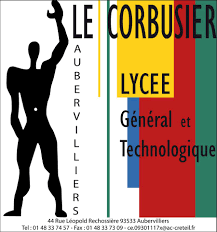
\includegraphics[height=23mm,keepaspectratio]{corbusier}} % Logo box - maximum height/width: 
}

%----------------------------------------------------------------------------------------
%	HEADER INFORMATION
%----------------------------------------------------------------------------------------
\fancyhead[L]{\begin{center}\textbf{Le Web}\end{center} \begin{tabular}{l r | l r} 
\textbf{Sujet} & Séquence : Le Web & SNT & V.Chevalier \\ 
\textbf{Seconde} & Sciences numériques \& technologie & 2021-2022 & Page : \thepage/\pageref{LastPage} \\ 
\end{tabular}}
%----------------------------------------------------------------------------------------





\begin{document}
%%%%%%%%%%%%%%%%%%%%%%%%%%%%%%%%%%POUR FAIRE UN COMPTEUR DE QUESTIONS%%%%%%%%%%%%%%%%%%%%%%%%%%%
\newcounter{question}
\newenvironment{question}{\stepcounter{question}\vspace{0.5cm}{\bfseries Question  \thequestion\   :  }}
%%%%%%%%%%%%%%%%%%%%%%%%%%%%%%%%%%POUR FAIRE UN COMPTEUR DE QUESTIONS%%%%%%%%%%%%%%%%%%%%%%%%%%%

\AddToShipoutPicture{\BackgroundStructure} % Set the background of each page to that specified above in the header information section

%----------------------------------------------------------------------------------------
%	DOCUMENT CONTENT
%----------------------------------------------------------------------------------------

\section{Séquence : Le web}
\subsection{Introduction et études préliminaires}

%%%%%%%%%%%%%%%%%%%%%%%%%%%%%%%%%%%%%%%%%%%%%%%%%%%%%%%%%%%%%%%%%%%%%%%%%%%%
\begin{figure}[!h!]
\centering
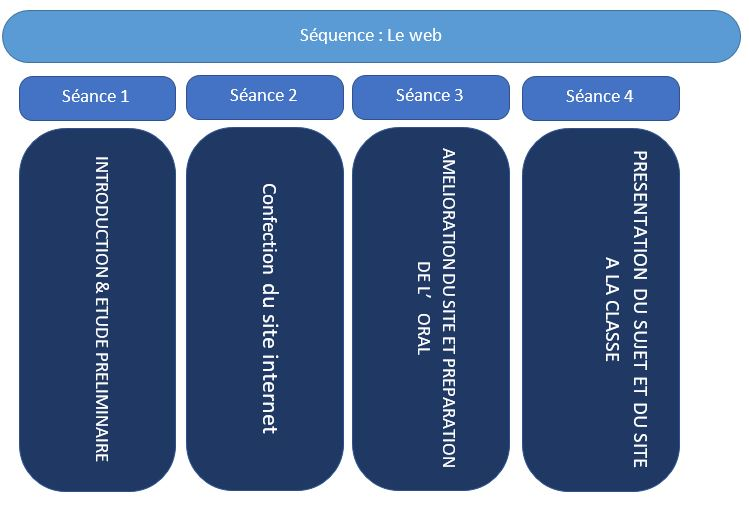
\includegraphics[scale=0.75]{1}
%\caption{Compléter le tableau en indiquant la valeur de l'angle $\alpha$ aux différents points A, B, C et D.}
\label{tableau1}
\end{figure}
%%%%%%%%%%%%%%%%%%%%%%%%%%%%%%%%%%%%%%%%%%%%%%%%%%%%%%%%%%%%%%%%%%%%%%%%%%%%%%

Étape de la séance 1 : 
\begin{enumerate}
\item Former des groupes de 3 élèves max;
\vspace{1cm}
\item Création d’un site internet sur les sujets suivants :


\begin{itemize}
\item Développement durable;
\item Nouvelles technologies;
\item Être lycéen.ne aujourd'hui;
\end{itemize}
\vspace{1cm}
\item Pourquoi faire ce site internet en particulier ? Qu’est-ce qui vous a fait choisir ce sujet;


\begin{tikzpicture}
\draw [very thick] (10,0) -- (23,0);
\draw [very thick] (10,4) -- (23,4);
\draw [very thick] (10,0) -- (10,4);
\draw [very thick] (23,0) -- (23,4);
\end{tikzpicture}



\item Quelles informations pourra-t-on trouver sur votre site ?


\begin{tikzpicture}
\draw [very thick] (10,0) -- (23,0);
\draw [very thick] (10,4) -- (23,4);
\draw [very thick] (10,0) -- (10,4);
\draw [very thick] (23,0) -- (23,4);
\end{tikzpicture}



\item Faire des recherches internet pour voir si l’idée de votre site n’est pas surreprésentée sur internet;
\vspace{1cm}
\item Etudier et choisir quelle sera votre public cible ? (Élèves, enseignants, salarié du développement durable, les parents d’élèves, etc.)

\begin{tikzpicture}
\draw [very thick] (10,0) -- (23,0);
\draw [very thick] (10,4) -- (23,4);
\draw [very thick] (10,0) -- (10,4);
\draw [very thick] (23,0) -- (23,4);
\end{tikzpicture}



\item Trouver un nom de domaine ! Il ne faut pas négliger cette étape car vous ne pourrez/devrez plus en changer. Si votre site est une marque, alors vous pouvez/devez prendre le nom de cette marque si le domaine est disponible. 


\vspace{0.5cm}
 Choisissez un nom de domaine qui soit :

\begin{itemize}
\item simple à retenir pour vos lecteur
\item  facilement identifiable
\item pas trop long. Idéalement, un nom de domaine doit comporter un mot ou des mots clés représentatifs de votre activité.
\item facilement référencable (si le mot clé peut être inclus dans le nom de domaine c'est mieux !)- un minimum marketable !
\end{itemize}


\begin{tikzpicture}
\draw [very thick] (10,0) -- (23,0);
\draw [very thick] (10,2) -- (23,2);
\draw [very thick] (10,0) -- (10,2);
\draw [very thick] (23,0) -- (23,2);
\end{tikzpicture}


\end{enumerate}

Si l'enseignant à validé tous les points avec vous, l'étape suivante sera :\\
\begin{itemize}
\item Commencer le design de votre futur site internet (maquette)

\item Chaque groupe présentera son sujet à la classe. A la fin de la séquence, chaque groupe présentera son site ainsi que son sujet. Les élèves de la classe poseront des questions sur le sujet. 

\item Chaque élève mettra une note qui comptera pour 25$\%$ de la note
\end{itemize}








%----------------------------------------------------------------------------------------

\end{document}